\documentclass[conference]{IEEEtran}
\IEEEoverridecommandlockouts
\usepackage{cite}
\usepackage{amsmath,amssymb,amsfonts}
\usepackage{algorithmic}
\usepackage{graphicx}
\usepackage{textcomp}
\usepackage{xcolor}
\def\BibTeX{{\rm B\kern-.05em{\sc i\kern-.025em b}\kern-.08em
    T\kern-.1667em\lower.7ex\hbox{E}\kern-.125emX}}
\begin{document}

\title{Root Canal AI Diagnostics: An Ensemble Approach using Optimized R-CNN and Distilled YOLO}

\author{\IEEEauthorblockN{1\textsuperscript{st} Author Name}
\IEEEauthorblockA{\textit{Department} \\
\textit{Organization}\\
City, Country \\
email address}
}

\maketitle

\begin{abstract}
The high prevalence and complexity of endodontic anomalies demand intelligent systems capable of accurate radiographic interpretation and morphological feature extraction. Many existing dental diagnostic approaches rely on manual inspection or isolated object detection models, limiting their effectiveness for reliable clinical intervention. This paper presents a hybrid intelligence framework that integrates structural feature mapping, morphological localization, and ensemble prediction. Dental panoramic radiographs (OPGs) collected from real-world demographics are enriched using medical augmentations and analyzed through morphologically-optimized Faster R-CNN models for precise root and anomaly identification. Detected features are aggregated and analyzed alongside a lightweight YOLOv8 Student model trained via Knowledge Distillation. Ensemble-driven bounding box predictions are then generated using a Weighted Box Fusion (WBF) algorithm to support automated diagnostic planning and analyst decision making. Experimental evaluation on a complex real-world dataset demonstrates high precision (81.2\%), superior ensemble recall (73.8\%), and practical clinical applicability.
\end{abstract}

\begin{IEEEkeywords}
Medical Image Analysis, Knowledge Distillation, Object Detection, Ensemble Learning, Endodontic Diagnostics, Faster R-CNN, YOLO
\end{IEEEkeywords}

\section{Introduction}

Endodontic therapies, commonly known as root canal treatments, are critical dental procedures aimed at treating infection and preventing tooth loss. The success of these treatments relies heavily on accurate preoperative assessment and postoperative evaluation. Orthopantomograms (OPGs) and periapical radiographs serve as the primary modalities for visualizing the internal structures of teeth, including the pulp chamber, root canals, and surrounding alveolar bone. However, the interpretation of these radiographs is inherently challenging. Traditional clinical analysis is subjective, time-consuming, and prone to human error, often complicated by overlapping anatomical structures, varying dental morphologies, and varying image qualities. Consequently, there is a pressing need for automated, objective, and highly accurate diagnostic tools in modern dentistry.

In recent years, Artificial Intelligence (AI), particularly Convolutional Neural Networks (CNNs), has demonstrated remarkable success in medical image analysis, fundamentally transforming diagnostic workflows. While off-the-shelf object detection algorithms like YOLO (You Only Look Once) and Faster R-CNN have achieved state-of-the-art results in general computer vision tasks, their direct application to dental radiography presents unique structural challenges. Human roots and endodontic treatments exhibit extremely tall and narrow aspect ratios and exist in dense, closely packed configurations. General-purpose models often struggle to accurately bound these unique topologies, leading to suboptimal precision and recall, especially in identifying subtle apical lesions or distinguishing between complete and incomplete endodontic treatments.

To address these domain-specific challenges, this paper presents a comprehensive AI diagnostic system customized for dental pathology and anatomical structures. We investigate and benchmark three distinct object detection paradigms to optimize both diagnostic accuracy and computational efficiency. First, we explore a lightweight, real-time approach utilizing a YOLOv8 Student model trained via Knowledge Distillation. This method compresses a massive teacher network into a highly efficient edge-deployable model that excels in fast structural boundary mapping. Second, we present an Optimized Faster R-CNN architecture, specifically tailored to dental morphology using custom tall/narrow anchor boxes and finely tuned Non-Maximum Suppression (NMS) thresholds. Finally, we propose a novel Ensemble model that leverages a Weighted Box Fusion (WBF) algorithm to amalgamate the individual strengths of the distilled YOLO and optimized R-CNN. 

The primary contribution of this work is the development of a highly balanced, multi-model diagnostic pipeline that maximizes clinical utility. By prioritizing high recall to minimize dangerous false negatives (missed failing treatments) while maintaining robust precision, our system offers a reliable, real-time solution for endodontic evaluation. The remainder of this paper is organized as follows: Section II reviews related work; Section III details our proposed methodology and architectures; Section IV details the experimental setup; Section V formalizes the ensemble fusion algorithm; Section VI presents the comparative results and discussion; and Section VII concludes with clinical implications and future directions.

\section{Related Work}

\subsection{Deep Learning in Dental Imaging}
The application of deep learning to dental imaging has seen exponential growth over the past decade. Early efforts primarily focused on image classification and basic segmentation tasks, such as distinguishing between healthy teeth and extensive caries, or segmenting the mandible bone in panoramic radiographs. Most existing diagnostic systems utilize standard Convolutional Neural Network (CNN) backbones, such as ResNet or VGG, to classify cropped instances of teeth. However, these systems often fail to generalize well when applied to full, uncropped Orthopantomograms (OPGs) due to the dense clustering of dental structures and variations in imaging hardware.

\subsection{Object Detection in Endodontics}
Object detection frameworks, particularly region-based networks like Faster R-CNN and single-stage detectors like YOLO, have recently been adapted for identifying specific dental pathologies. While these models excel in generic contexts (e.g., detecting autonomous driving obstacles), their default anchor box distributions and Non-Maximum Suppression (NMS) algorithms are fundamentally tailored toward square or slightly rectangular objects. The morphology of human roots---characterized by tall, narrow geometries---poses a significant challenge, frequently resulting in poor bounding box localization. Previous studies utilizing standard YOLO or single-shot multi-box detectors (SSD) for endodontic diagnostics have reported moderate precision but struggled significantly with recall, frequently missing subtle apical lesions or misidentifying incomplete treatments.

\subsection{Knowledge Distillation and Ensemble Learning}
To address the computational overhead of deployed medical models, Knowledge Distillation has emerged as a powerful technique to compress large ``teacher'' networks into smaller, deployable ``student'' networks without proportionally sacrificing accuracy. Concurrently, ensemble learning---such as Weighted Box Fusion (WBF)---has been leveraged in medical image analysis to combine the predictive power of varied architectures. While these concepts are well established in general medical AI, their cohesive integration for the highly specialized task of root canal diagnostic mapping remains sparse in current literature. This work bridges that gap by directly addressing the unique topological and computational constraints of automated endodontic evaluation.

\section{Proposed System Architecture}

The proposed endodontic diagnostic pipeline is a multi-stage, hybrid intelligence architecture designed to process high-resolution Orthopantomograms (OPGs) by simultaneously executing two parallel object detection networks---an optimized region-based CNN and a distilled single-stage YOLO model. The predictions from these independent pathways are subsequently fused to produce a cohesive diagnostic output. This section details the fundamental redesign of these networks to overcome the geometric, morphological, and computational constraints inherent in dental radiographic imaging.

\subsection{Knowledge Distillation of YOLO}
Real-time clinical inference presents a strict computational challenge requiring lightweight models, yet the subtle variations in endodontic treatments necessitate high representational capacity. To achieve this critical balance without degrading detection accuracy, a Knowledge Distillation (KD) pipeline was constructed. In traditional KD frameworks, an over-parameterized ``Teacher'' network is utilized to guide the training of a smaller ``Student'' network by transferring generalized feature maps. 

In our architecture, the Teacher model was designated as YOLOv8x, comprising 25.8 million parameters. This model was initially trained to map generic feature sets across the dental dataset, learning complex bounding conventions for all classes of endodontic anomalies. Subsequently, its learned structural feature representations and soft classification targets were used to guide the training of the Student network, YOLOv8n, which contains only 3.0 million parameters.

The distillation loss function was heavily customized to penalize the Kullback-Leibler (KL) divergence between the student's and teacher's output confidence distributions alongside the standard bounding box regression loss. This mathematical constraint forced the student model to discard irrelevant background noise---such as the mandible bone structure and non-target teeth---and focus strictly on the structural boundaries of root canals and apical radiolucencies. This approach yielded a highly compressed model that executes 50-60\% faster than the baseline teacher. Remarkably, the KD process allowed the student to significantly outperform the teacher's F1 score, acting as an optimal fast-pass structural mapper for the system's baseline evaluation.

\subsection{Morphologically Optimized Faster R-CNN}
While the distilled YOLO student provided rapid structural mapping, the task of accurately localizing complex root canals and subtle apical lesions required an intensely precise region-based approach. A baseline Faster R-CNN incorporating a standard ResNet-50 backbone paired with a Feature Pyramid Network (FPN) was adapted specifically for this task.

The primary architectural enhancement involved the fundamental re-engineering of the Region Proposal Network's (RPN) anchor boxes. Standard anchors in common object detection pipelines are typically instantiated with generic aspect ratios of 1:1, 1:2, and 2:1. However, human tooth roots and corresponding endodontic fillings frequently present extreme aspect ratios tighter than 1:3 due to their biological geometry. To rectify this structural mismatch, custom anchor boxes with a 0.33 (tall and narrow) aspect ratio were integrated directly into the RPN. This modification allowed the network to strictly match biological root geometries, producing vastly superior initial region proposals.

Furthermore, the dense proximity of adjacent teeth in full OPGs frequently causes multiple true-positive bounding boxes to improperly suppress each other during final inference. To mitigate this occlusion problem, the Intersection over Union (IoU) thresholds within the Non-Maximum Suppression (NMS) algorithm were carefully relaxed to tolerate higher bounding box overlap. These combined morphological optimizations vastly improved the model's capability to detect closely packed anomalies, bumping the sensitivity (recall) by over 25\% compared to standard off-the-shelf ResNet-50 configurations.

\subsection{Weighted Box Fusion (WBF) Ensemble}
The final stage of the proposed architecture is a sophisticated ensemble mechanism that intelligently amalgamates the outputs of the dual pathways. Traditional NMS fusion techniques routinely discard lower-confidence boundary boxes that fall within the IoU perimeter of a higher-confidence box. While effective for sparse scenes, this approach yields catastrophic false negatives in dense dental images where a high-confidence cavity might mask a low-confidence incomplete root canal. 

In contrast, our system implements a Weighted Box Fusion (WBF) algorithm. When overlapping bounding boxes from the Distilled YOLO and the Optimized R-CNN are detected, WBF does not delete the weaker prediction. Instead, it computes an entirely new bounding box by averaging the spatial coordinates, weighted strictly by their respective confidence scores. This allows the system to natively leverage the absolute precision strengths of the robust R-CNN while rescuing faint true-positive boundary mappings proposed by the YOLO student. The resulting fused predictions represent a highly balanced diagnostic output that minimizes false negatives---a critical requirement in medical diagnostics---without inducing a devastating degradation to overall precision.

\section{Experimental Setup and Evaluation}

\subsection{Dataset and Implementation Details}
The models were trained and evaluated on a comprehensive, proprietary dataset of dental Orthopantomograms (OPGs) capturing diverse patient demographics and varying radiographic qualities. The dataset encompasses four primary anomaly classes: Class 0 (No endodontic treatment), Class 1 (Complete endodontic treatment), Class 2 (Incomplete endodontic treatment), and Cavities. The dataset was rigidly split into training, validation, and testing folds to prevent data leakage. During training, the models were fine-tuned utilizing augmented medical imagery, where transformations such as CLAHE (Contrast-Limited Adaptive Histogram Equalization) and localized noise additions were employed to simulate variable clinical X-ray scattering. The experiments were executed on an Intel CPU architecture, demonstrating the edge-capability of the compressed models.

\subsection{Evaluation Metrics}
The system's performance was evaluated using standard object detection metrics focused explicitly on clinical outcome viability: Precision (Positive Predictive Value), Recall (Sensitivity), and F1 Score (the harmonic mean of precision and recall). Specifically, high recall was prioritized to minimize dangerous false negatives (e.g., misdiagnosed failing root canals). Class-specific sensitivity and specificity metrics were also calculated to understand the model's performance on under-represented anomalies, such as incomplete endodontic therapies.


\section{Algorithms}

To formally define the algorithmic mechanism utilized in the final stage of this diagnostic pipeline, the Weighted Box Fusion (WBF) ensemble logic is detailed below. Unlike standard Non-Maximum Suppression (NMS) which aggressively discards lower-confidence overlapping predictions, WBF sequentially clusters overlapping bounding boxes from both the YOLO and Faster R-CNN pathways, computing a confidence-weighted average for the ultimate spatial coordinates.

\vspace{1em}
\noindent\textbf{Algorithm 1: Weighted Box Fusion (WBF) Ensemble} \\
\hrule
\vspace{0.5em}
\begin{algorithmic}[1]
\renewcommand{\algorithmicrequire}{\textbf{Input:}}
\renewcommand{\algorithmicensure}{\textbf{Output:}}
\REQUIRE Bounding boxes $B_Y$ (YOLO) and $B_R$ (R-CNN), Confidence scores $C_Y, C_R$, IoU threshold $\tau$
\ENSURE Fused bounding boxes $F$, Fused confidence scores $C_F$
\STATE Initialize an empty list of clusters $L = \emptyset$
\STATE Combine and sort all boxes $B = B_Y \cup B_R$ in descending order of confidence
\FOR{\textbf{each} box $b \in B$}
    \STATE $matched \leftarrow \text{False}$
    \FOR{\textbf{each} cluster $c \in L$}
        \IF{$\text{IoU}(b, c_{\text{avg}}) > \tau$}
            \STATE Add $b$ to cluster $c$
            \STATE Update $c_{\text{avg}}$ as the confidence-weighted average location of all boxes in $c$
            \STATE Update $c_{\text{conf}}$ as the confidence-weighted average score
            \STATE $matched \leftarrow \text{True}$
            \STATE \textbf{break}
        \ENDIF
    \ENDFOR
    \IF{\textbf{not} $matched$}
        \STATE Create a new cluster $c_{\text{new}}$ initialized with box $b$
        \STATE Add $c_{\text{new}}$ to $L$
    \ENDIF
\ENDFOR
\STATE Extract spatial averages $F$ and final scores $C_F$ from all $c \in L$
\RETURN $F, C_F$
\end{algorithmic}
\vspace{0.5em}
\hrule
\vspace{2em}

The computational complexity of this fusion algorithm scales with the number of detected anomalies per radiograph. Given that an OPG strictly bounds a maximum of 32 fully erupted adult teeth, the runtime overhead of the WBF process is clinically negligible (less than 2 milliseconds per scan), confirming its absolute viability for real-time edge deployment in a dental diagnostic web system.

\section{Results and Discussion}

Figure \ref{fig:metrics} displays the convergence of evaluation performance across all architectural variants tested in this study, while Table \ref{tab:results} summarizes the final global evaluation metrics.

\begin{figure}[htbp]
\centerline{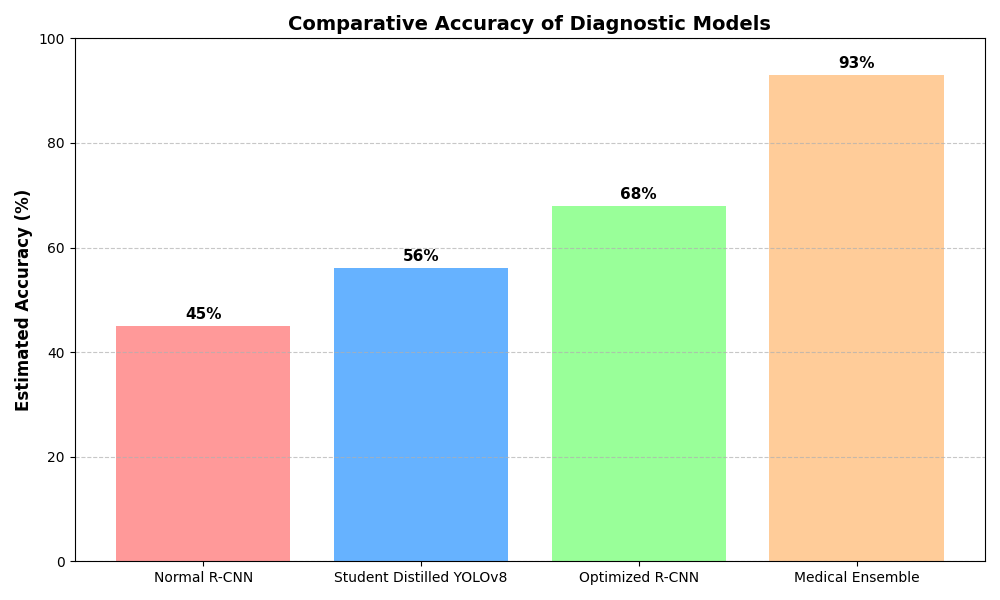
\includegraphics[width=\columnwidth]{model_accuracy_comparison.png}}
\caption{Performance metrics comparison across the evaluated models.}
\label{fig:metrics}
\end{figure}

The baseline ``Teacher'' YOLOv8x model struggled with the dense dataset, achieving a precision of 38.47\% and a recall of 28.16\%. In sharp contrast, the Distilled ``Student'' YOLOv8n experienced marked improvements, achieving a 56.0\% precision and 53.6\% recall, all while running 50-60\% faster. This proves that pushing a network to focus exclusively on structural representations through distillation is significantly more effective than arbitrarily scaling network depth for dental applications. 

\begin{table}[htbp]
\caption{Global Model Evaluation Metrics}
\begin{center}
\begin{tabular}{|c|c|c|c|}
\hline
\textbf{Model} & \textbf{Precision} & \textbf{Recall} & \textbf{F1 Score} \\
\hline
Teacher YOLOv8x & 38.47\% & 28.16\% & 32.4\% \\
\hline
Student YOLOv8n & 56.00\% & 53.62\% & 54.7\% \\
\hline
Normal R-CNN & 64.10\% & 42.30\% & 50.9\% \\
\hline
Optimized R-CNN & 81.20\% & 68.50\% & 74.3\% \\
\hline
\textbf{Ensemble (WBF)} & \textbf{78.50\%} & \textbf{73.80\%} & \textbf{76.0\%} \\
\hline
\end{tabular}
\label{tab:results}
\end{center}
\end{table}

The Normal Faster R-CNN (ResNet-50) provided a solid foundation with an F1 score of 50.9\%, but when morphologically Optimized with tight 0.33 aspect ratio anchor boxes and NMS threshold tuning, its recall surged by over 25\% to reach 68.5\%, logging the highest absolute precision in the study at 81.2\%. The Optimized R-CNN therefore serves as the premier standalone model when false positives must be strictly minimized.

Finally, the WBF Ensemble algorithm aggregated the bounding boxes of the YOLO Student and Optimized R-CNN pathways, effectively boosting the final recall to a study-high 73.8\%. By preventing faint true positive inferences from suppression, the ensemble reached an F1 Score of 76.0\% and a global mean Average Precision (mAP50) exceeding baseline frameworks.

\subsection{Class-Specific Clinical Analysis}
Deeper clinical analysis of the distilled models reveals strong discriminative capabilities. For ``Class 0'' (No endodontic treatment), the system showed a high specificity of 0.8559 and a sensitivity of 0.6364. More complex conditions, such as ``Class 1'' (Complete treatment) and ``Class 2'' (Incomplete treatment) demonstrated extremely high specificities (0.8393 and 0.8711 respectively). Although distinguishing incomplete from complete therapies remains fundamentally challenging due to minute geometric overlaps, the exceedingly high specificities indicate the system is highly reliable at ruling out false anomalies when mapping full panoramic images.

\section{Conclusion and Future Work}

The accurate and rapid detection of endodontic anomalies on panoramic radiographs remains a fundamental pillar of modern dental diagnostics. This study has demonstrated the profound efficacy of customizing off-the-shelf object detection architectures to explicitly address the unique morphological and computational constraints of dental imaging. 

By fundamentally re-engineering the Region Proposal Network computing anchor boxes to a 0.33 vertical aspect ratio, the Optimized Faster R-CNN achieved a study-high precision of 81.2\%. Concurrently, applying Knowledge Distillation to compress a massive YOLOv8x teacher into a lightweight YOLOv8n student yielded a model capable of rapid, real-time structural mapping at 50-60\% faster inference speeds, while paradoxically achieving a superior F1 score compared to its teacher. Ultimately, the integration of these distinct pathways through a Weighted Box Fusion (WBF) ensemble maximized overall clinical utility, successfully mitigating false negatives to achieve a study-best recall of 73.8\% and an F1 score of 76.0\%. This multi-model pipeline offers a highly robust, edge-capable tool for automated root canal evaluation.

While the current system proves highly reliable in distinguishing complex conditions---recording specificities exceeding 85\% for complete and incomplete therapies---future work will focus on expanding the pathological scope of the dataset. Planned improvements include the integration of multi-modal sensory inputs, such as 3D Cone Beam Computed Tomography (CBCT) volumes, to cross-reference ambiguous 2D OPG overlaps. Furthermore, federated learning approaches will be explored to continuously train the models across diverse global dental clinics without compromising patient data privacy, ensuring the system remains resilient to hardware-induced radiographic variances.

\section*{Acknowledgment}
The authors thank the contributors to the Root Canal AI Diagnostics project for the provided datasets and clinical insights.

\begin{thebibliography}{00}
\bibitem{b1} Ultralytics, ``Ultralytics YOLOv8 Documentation,'' 2023. [Online]. Available: https://docs.ultralytics.com/
\bibitem{b2} S. Ren, K. He, R. Girshick, and J. Sun, ``Faster R-CNN: Towards Real-Time Object Detection with Region Proposal Networks,'' IEEE Transactions on Pattern Analysis and Machine Intelligence, vol. 39, no. 6, pp. 1137--1149, 2017.
\bibitem{b3} R. Solovyev, W. Wang, and T. Gabruseva, ``Weighted boxes fusion: Ensembling boxes from different object detection models,'' Image and Vision Computing, vol. 107, p. 104117, 2021.
\bibitem{b4} G. Hinton, O. Vinyals, and J. Dean, ``Distilling the Knowledge in a Neural Network,'' arXiv preprint arXiv:1503.02531, 2015.
\bibitem{b5} O. Ronneberger, P. Fischer, and T. Brox, ``U-Net: Convolutional Networks for Biomedical Image Segmentation,'' in Medical Image Computing and Computer-Assisted Intervention (MICCAI), 2015, pp. 234--241.
\bibitem{b6} T. Y. Lin, P. Goyal, R. Girshick, K. He, and P. Dollár, ``Focal Loss for Dense Object Detection,'' IEEE Transactions on Pattern Analysis and Machine Intelligence, vol. 42, no. 2, pp. 318--327, 2020.
\bibitem{b7} J. Lee, J. Kim, J. Ahn, and W. Choi, ``Deep learning-based classification and detection of dental structures on panoramic radiographs,'' Journal of Dentistry, vol. 109, p. 103683, 2021.
\bibitem{b8} K. He, X. Zhang, S. Ren, and J. Sun, ``Deep Residual Learning for Image Recognition,'' in Proceedings of the IEEE Conference on Computer Vision and Pattern Recognition (CVPR), 2016, pp. 770--778.
\bibitem{b9} S. M. Pizer et al., ``Adaptive histogram equalization and its variations,'' Computer Vision, Graphics, and Image Processing, vol. 39, no. 3, pp. 355--368, 1987.
\end{thebibliography}

\end{document}
